
\documentclass[handout]{beamer}
%%\usetheme{Warsaw}  %%Wählt das Layout der Präsentation aus
\usetheme{Boadilla}
%%\usetheme{Berlin}
%%\usetheme{boxes} %% ich mag Boadilla am liebsten, aber ihr könnt auch gerne was anderes vorschlagen

\usepackage[ngerman]{babel} 
\usepackage[utf8]{inputenc}
\usepackage{amsmath,amsfonts,amssymb}
\usepackage{graphicx}
\usepackage{svg}
\usepackage{listings}

\title[Aufgabe 4]{Aufgabe 4 des praktischen Übungsblatts}
\author[Schmidt, Pielka]{Christopher Schmidt, Maren Pielka}
\institute[Uni Bonn]{Universität Bonn}
\date[13.01.16]{13. Januar 2016}

\begin{document}

\begin{frame}
\titlepage
\end{frame}

\begin{frame}[containsverbatim]
\frametitle{Measurement setup}
\begin{itemize}
\item Durchführung aller Messungen auf Rechnern im CIP-Pool
\item \textit{wget} zum Herunterladen der Dateien, Auswertung und Plot mit Python-Skript
\lstset{language=sh,basicstyle=\footnotesize}
\begin{lstlisting}
$ wget -O - [...] | python exercise4v2.py
\end{lstlisting}
\item Download von "linux-3.9.2.tar.xz" (ca. 68 MB) zum Testen 
\end{itemize}
\end{frame}

\begin{frame}
\frametitle{HTTP Server Ergebnisse}
\begin{itemize}
\item Drosselung zu Beginn des Downloads
\end{itemize}

\begin{figure}
\centering
\begin{minipage}[t]{0.4\linewidth}
			\centering
			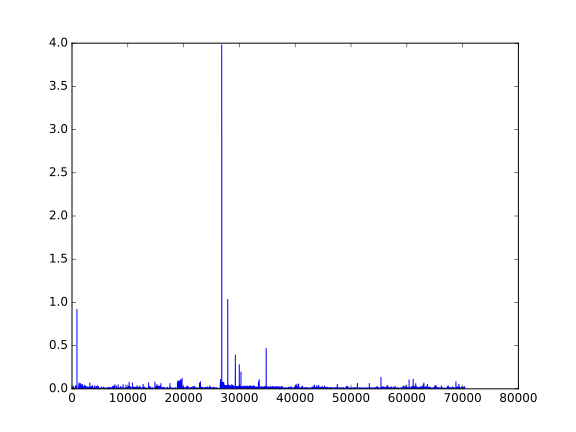
\includegraphics[width=\linewidth]{images/seconds_http.pdf}
			\caption{Zeit in Sekunden für je 1 KByte}
\end{minipage}
\begin{minipage}[t]{0.4\linewidth}
			\centering
			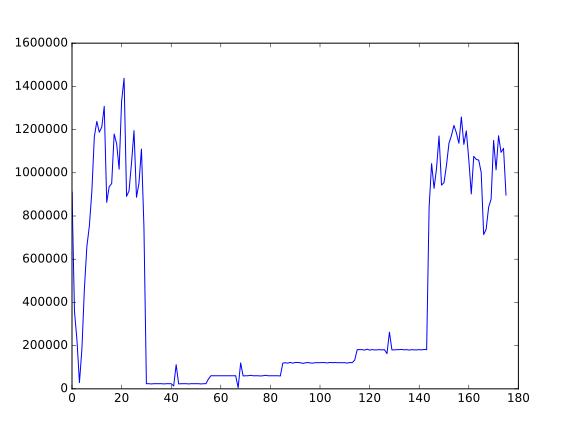
\includegraphics[width=\linewidth]{images/datarate_http.pdf}
			\caption{KByte pro Sekunde}
\end{minipage}
\end{figure}
\end{frame}

\begin{frame}
\frametitle{FTP Server Ergebnisse}
\begin{itemize}
\item Drosselung am Ende des Downloads
\end{itemize}
\begin{figure}
\centering
\begin{minipage}[t]{0.4\linewidth}
			\centering
			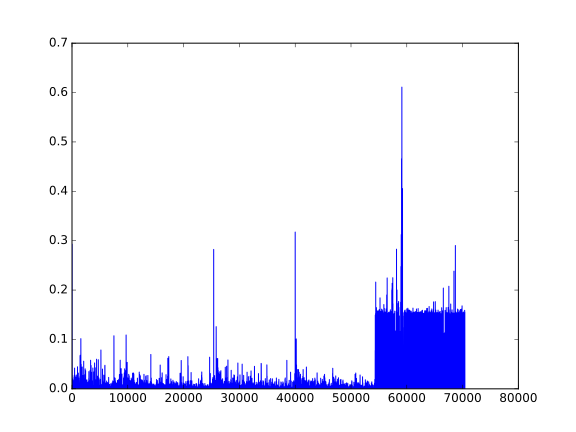
\includegraphics[width=\linewidth]{images/seconds_ftp.pdf}
			\caption{Zeit in Sekunden für je 1 KByte}
\end{minipage}
\begin{minipage}[t]{0.4\linewidth}
			\centering
			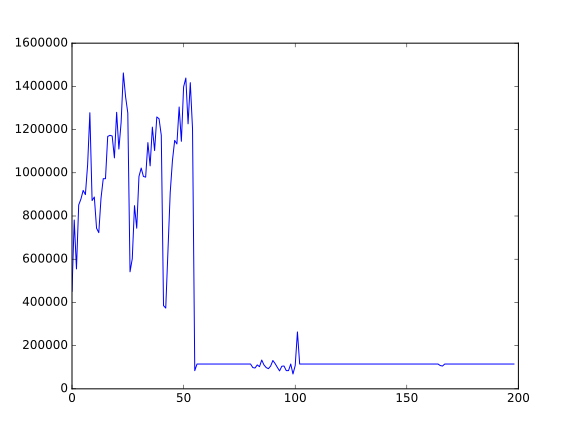
\includegraphics[width=\linewidth]{images/datarate_ftp.pdf}
			\caption{KByte pro Sekunde}
\end{minipage}
\end{figure}
\end{frame}

\end{document}